%#!uplatex main.tex

\section{Tessellation}

\emph{テセレーション}{\it (Tessellation)}
とは平面や空間を平面図形や空間図形で埋め合わせることをいう.
これは\emph{タイリング}{\it(Tiling)}ともよばれる.
図\ref{fig:rightTriangular}は直角二等辺三角形を各辺における鏡映変換で移
すことで平面を敷き詰めた模様を描いた.
図\ref{fig:tessellationT}はアルファベットのTによる敷き詰め模様を描いた.
こうした敷き詰め模様は装飾として太古から親しまれており,アートとしても非常に人気のある分野である.
クライン群の図でも様々なところに敷き詰め模様を見ることができる.
例えば図\ref{fig:schottky}は黒の基本領域を周囲の円盤の反転で移した敷き詰
め模様と捉えることができる.

ユークリッド平面上での敷き詰め模様は,数学的に分類がされている.
この分類に関しては『装飾パターンの法則』
\cite{fujitaー201507pattern}が詳しい.
この本は主にデザイナーに向けて,装飾に用いられる敷き詰め模様の法則性と
分類について記述しており,敷き詰め模様のデザインへの応用に役立つ.
敷き詰めの分類がより専門的にまとめられた文献にはMartin von Gagern,Jrgen
Richter-Gebertによる\cite{journals/combinatorics/GagernR09}がある.
この論文はユークリッド平面上での敷き詰め模様を双曲平面での敷き詰めに変換
する方法を提案したものであるが,敷き詰め模様の分類についても詳しい.
また,Gagernによる\emph{morenaments}\footnote{morenaments:~
\url{http://www.morenaments.de/}}というソフトウェアを用いることで,各敷
き詰めパターンの挙動をみることができる.

\begin{figure}[h!tbp]
 \begin{minipage}{0.49\hsize}
  \center
  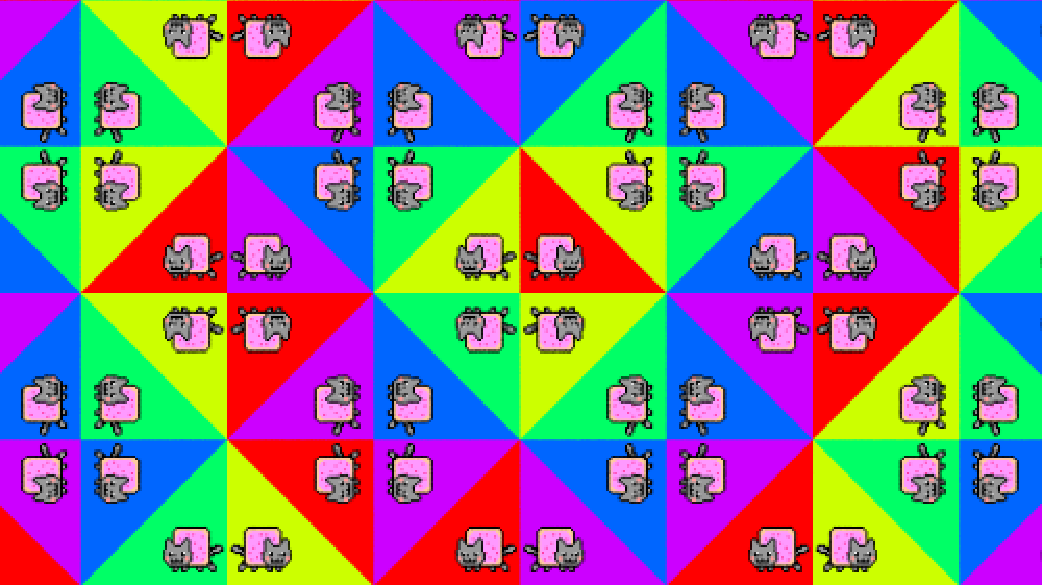
\includegraphics[width=3in, height=3in, keepaspectratio]{../img/tessellation/rightTriangular.pdf}
  \caption{Right triangular tiling}
  \label{fig:rightTriangular}
 \end{minipage}
 \begin{minipage}{0.49\hsize}
  \center
  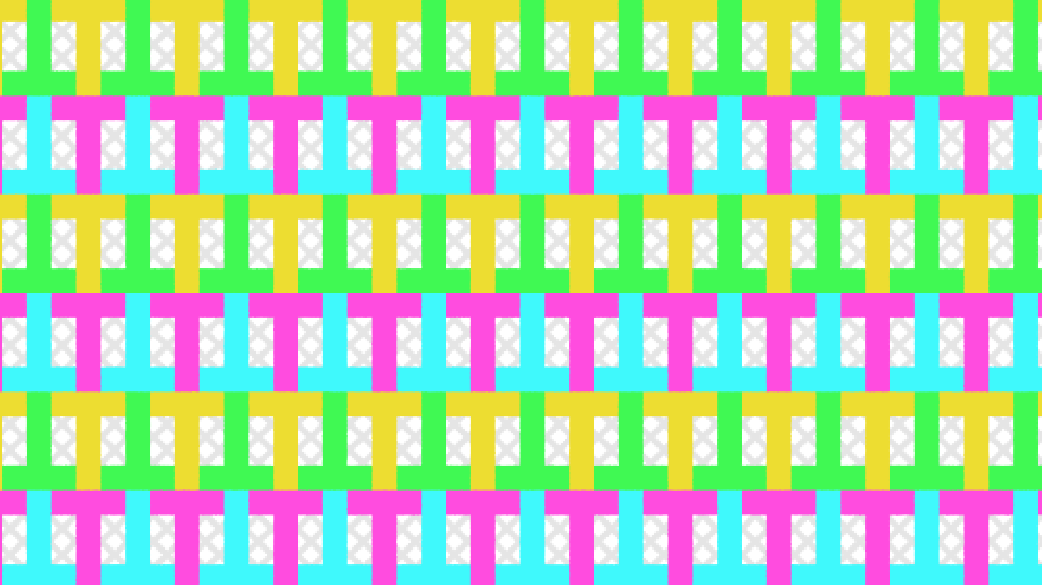
\includegraphics[width=3in, height=3in, keepaspectratio]{../img/tessellation/tessellationT.pdf}
  \caption{Tessellation of alphabet T}
  \label{fig:tessellationT}
 \end{minipage}
\end{figure}

\subsection{About Rendering}

敷き詰め模様をシェーダを用いて描画することを考えるため,
まずは図\ref{fig:rectTile}のような正方形のテセレーションを
考える.基本的には図\ref{fig:tile}に矢印で示されるような,縦横全4種類の
変換の組み合わせで基本となる正方形を動かすことで,平面全体を正方形で埋め
尽くすことができる.
シェーダを使わない場合,前章でみた群の軌道の描画方法と同様に,変換の木構
造を幅優先探索し,得られた合成変換で正方形を移動させることでこれを描画す
ることができる.
一方で,シェーダを用いて描画する場合にはその逆の操作を行う.
すなわち,図\ref{fig:tileMove}のように各ピクセルを,敷き詰めを構成する4種
の変換で基本タイルへと点を動かす.
そうして,基本タイルへ動かした後で操作の回数や基本タイル上の色からそのピ
クセルの色を決めて塗る.
これはおおむねIISと同様のアプローチである.
ただし,この方法ではペンローズタイリングのような非周期的な敷き詰め模様を
描くことは難しい.このアルゴリズムをまとめると以下のような手順になる.
\begin{enumerate}
 \item 基本タイルを見つける.
 \item 基本タイルを敷き詰めるための変換を見つける.
 \item 各ピクセルを基本タイルに入るまで変換し続ける.
 \item 変換の回数や基本タイル上の色を使って色を付ける.
\end{enumerate}
正方形によるタイリングにおける変換の回数を計算するための擬似コードをアル
ゴリズム\ref{alg:rectTile}に示した.
このアルゴリズムによって得られた回数によって色をつけることで正方形の敷き詰め模
様を見ることができる.例えば,偶数回の操作と奇数回の操作で白と黒に分けれ
ばチェッカーボード模様が得られる.また,この操作も剰余を用いて最適化
することができる.

\begin{figure}[h!tbp]
 \begin{subfigure}{0.3\textwidth}
  \center
  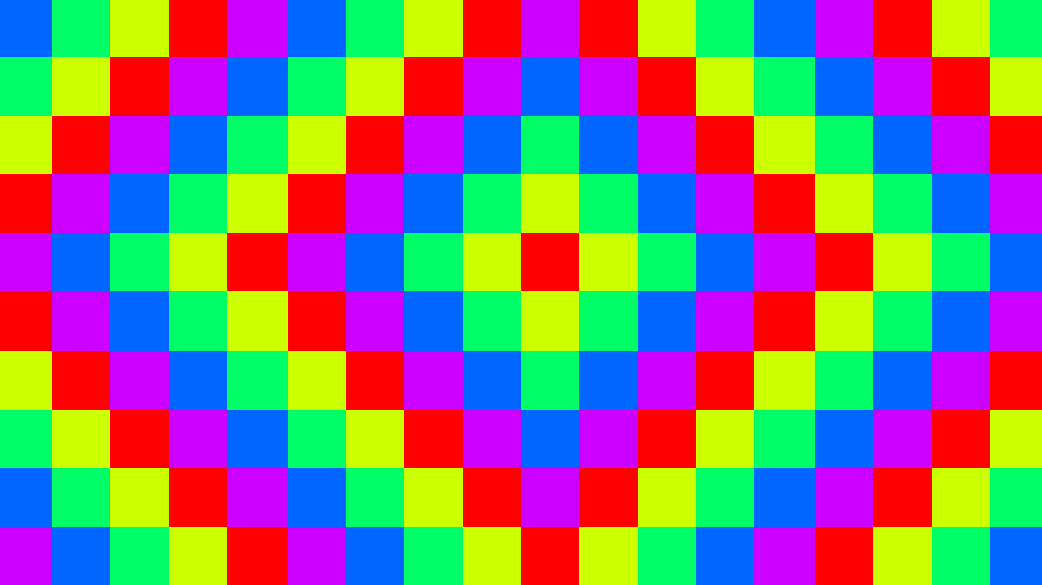
\includegraphics[width=2in, height=2in, keepaspectratio]{../img/tessellation/rectTile.pdf}
  \caption{Square tiling}
  \label{fig:rectTile}
 \end{subfigure}
 \hspace*{\fill}
 \begin{subfigure}{0.3\textwidth}
  \center
  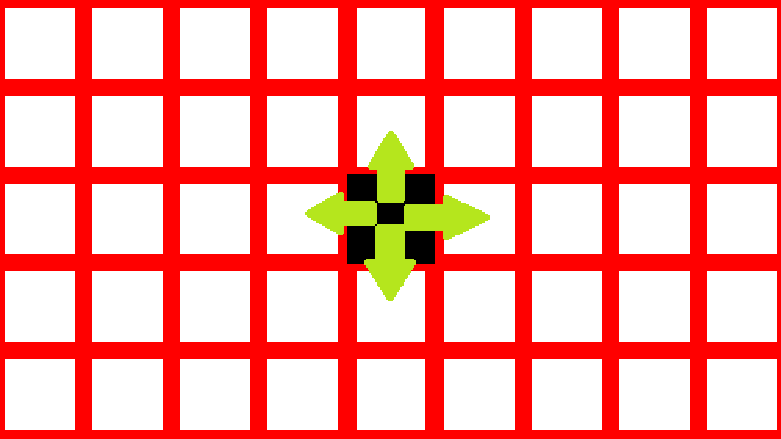
\includegraphics[width=2in, height=2in, keepaspectratio]{../img/tessellation/tile.pdf}
  \caption{Tile and transformations}
  \label{fig:tile}
 \end{subfigure}
 \hspace*{\fill}
 \begin{subfigure}{0.3\textwidth}
  \center
  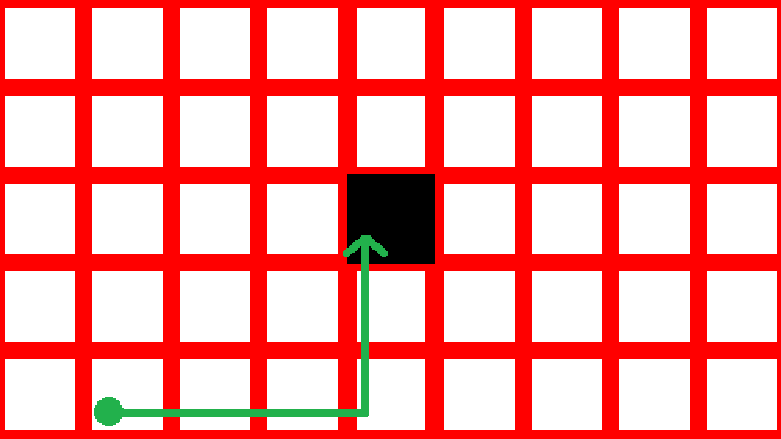
\includegraphics[width=2in, height=2in, keepaspectratio]{../img/tessellation/tileMove.pdf}
  \caption{Move}
  \label{fig:tileMove}
 \end{subfigure}
 \hspace*{\fill}
\caption{Tile}
\end{figure}

\begin{algorithm}
 \begin{algorithmic}
  \caption{Count number of operations for square tiling}
  \label{alg:rectTile}
  \REQUIRE count $= 0$ and coordinates $=$ position determined by pixel
  \FOR{$i=0$ to \texttt{MAX\char`_INVERSION}}
  \STATE inFundamentalDomain $\leftarrow$ \TRUE
  \IF{coordinates.x $< 0$}
  \STATE coordinates.x $\leftarrow$ coordinates.x + \texttt{SQUARE\char`_SIZE}
  \STATE INCREMENT count
  \STATE inFundamentalDomain $\leftarrow$ \FALSE
  \ENDIF
  \IF{coordinates.x $>$ \texttt{SQUARE\char`_SIZE}}
  \STATE coordinates.x $\leftarrow$ coordinates.x - \texttt{SQUARE\char`_SIZE}
  \STATE INCREMENT count
  \STATE inFundamentalDomain $\leftarrow$ \FALSE
  \ENDIF
  \IF{coordinates.y $< 0$}
  \STATE coordinates.y $\leftarrow$ coordinates.y + \texttt{SQUARE\char`_SIZE}
  \STATE INCREMENT count
  \STATE inFundamentalDomain $\leftarrow$ \FALSE
  \ENDIF
  \IF{coordinates.y $>$ \texttt{SQUARE\char`_SIZE}}
  \STATE coordinates.y $\leftarrow$ coordinates.y - \texttt{SQUARE\char`_SIZE}
  \STATE INCREMENT count
  \STATE inFundamentalDomain $\leftarrow$ \FALSE
  \ENDIF
  \IF {inFundamentalDomain}
  \STATE BREAK for
  \ENDIF
  \ENDFOR
  \STATE RETURN count
 \end{algorithmic}
\end{algorithm}

\subsection{Hyperbolic Tessellation}

我々が普段見ている世界を考えるユークリッド幾何学では,平面上に任意の直線
$L$とその直線上にない点$P$があるとき,$P$を通り,$L$に平行な直線は一本しか
引くことができない.
これは\emph{平行線公準}とよばれている.
ボヤイ(Bolyai),ロバチェフスキー(Lobachevsky),ガウス(Gauss)といった数学者は,
こういった公理を崩した幾何学のモデルの一つである\emph{双曲幾何
学}(\textit{Hyperbolic Geometry})を考案した.
双曲幾何学では$L$に平行な直線を無限に引くことができる.
また,最も特徴的なのは三角形の内角の和が180度以下になるということである.

双曲幾何学における平面は我々が普段考える平面とは異なるものとなる.
そのモデルとして有名なものに\emph{ポアンカレの円盤モデ
ル}(\textit{Poincar\'e disk model})や\emph{ポアンカレの上半平面モデ
ル}(\textit{Poincar\'e half-plane model})がある.
図\ref{fig:hyperbolicTessellation}に円盤モデルと上半平面モデルにおけるテ
セレーションを示した.
双曲幾何学における平面である双曲平面の敷き詰め模様は,\emph{双曲テセ
レーション}{\it (Hyperbolic Tessellation)}とよばれる.
画家のM.C.エッシャーはこのような図に影響されて『天使と悪魔』や『Circle
Limit』といった有名な作品を生み出した.
円盤モデルにおいては図\ref{fig:disk}に示される円盤が双
曲平面であり,世界のすべてである.
円盤の端がユークリッド平面における無限遠点となる.
また,双曲平面では円弧が直線となり,あらゆるタイルが円弧で構成される.

\begin{figure}[h!tbp]
 \begin{minipage}{0.49\hsize}
  \center
  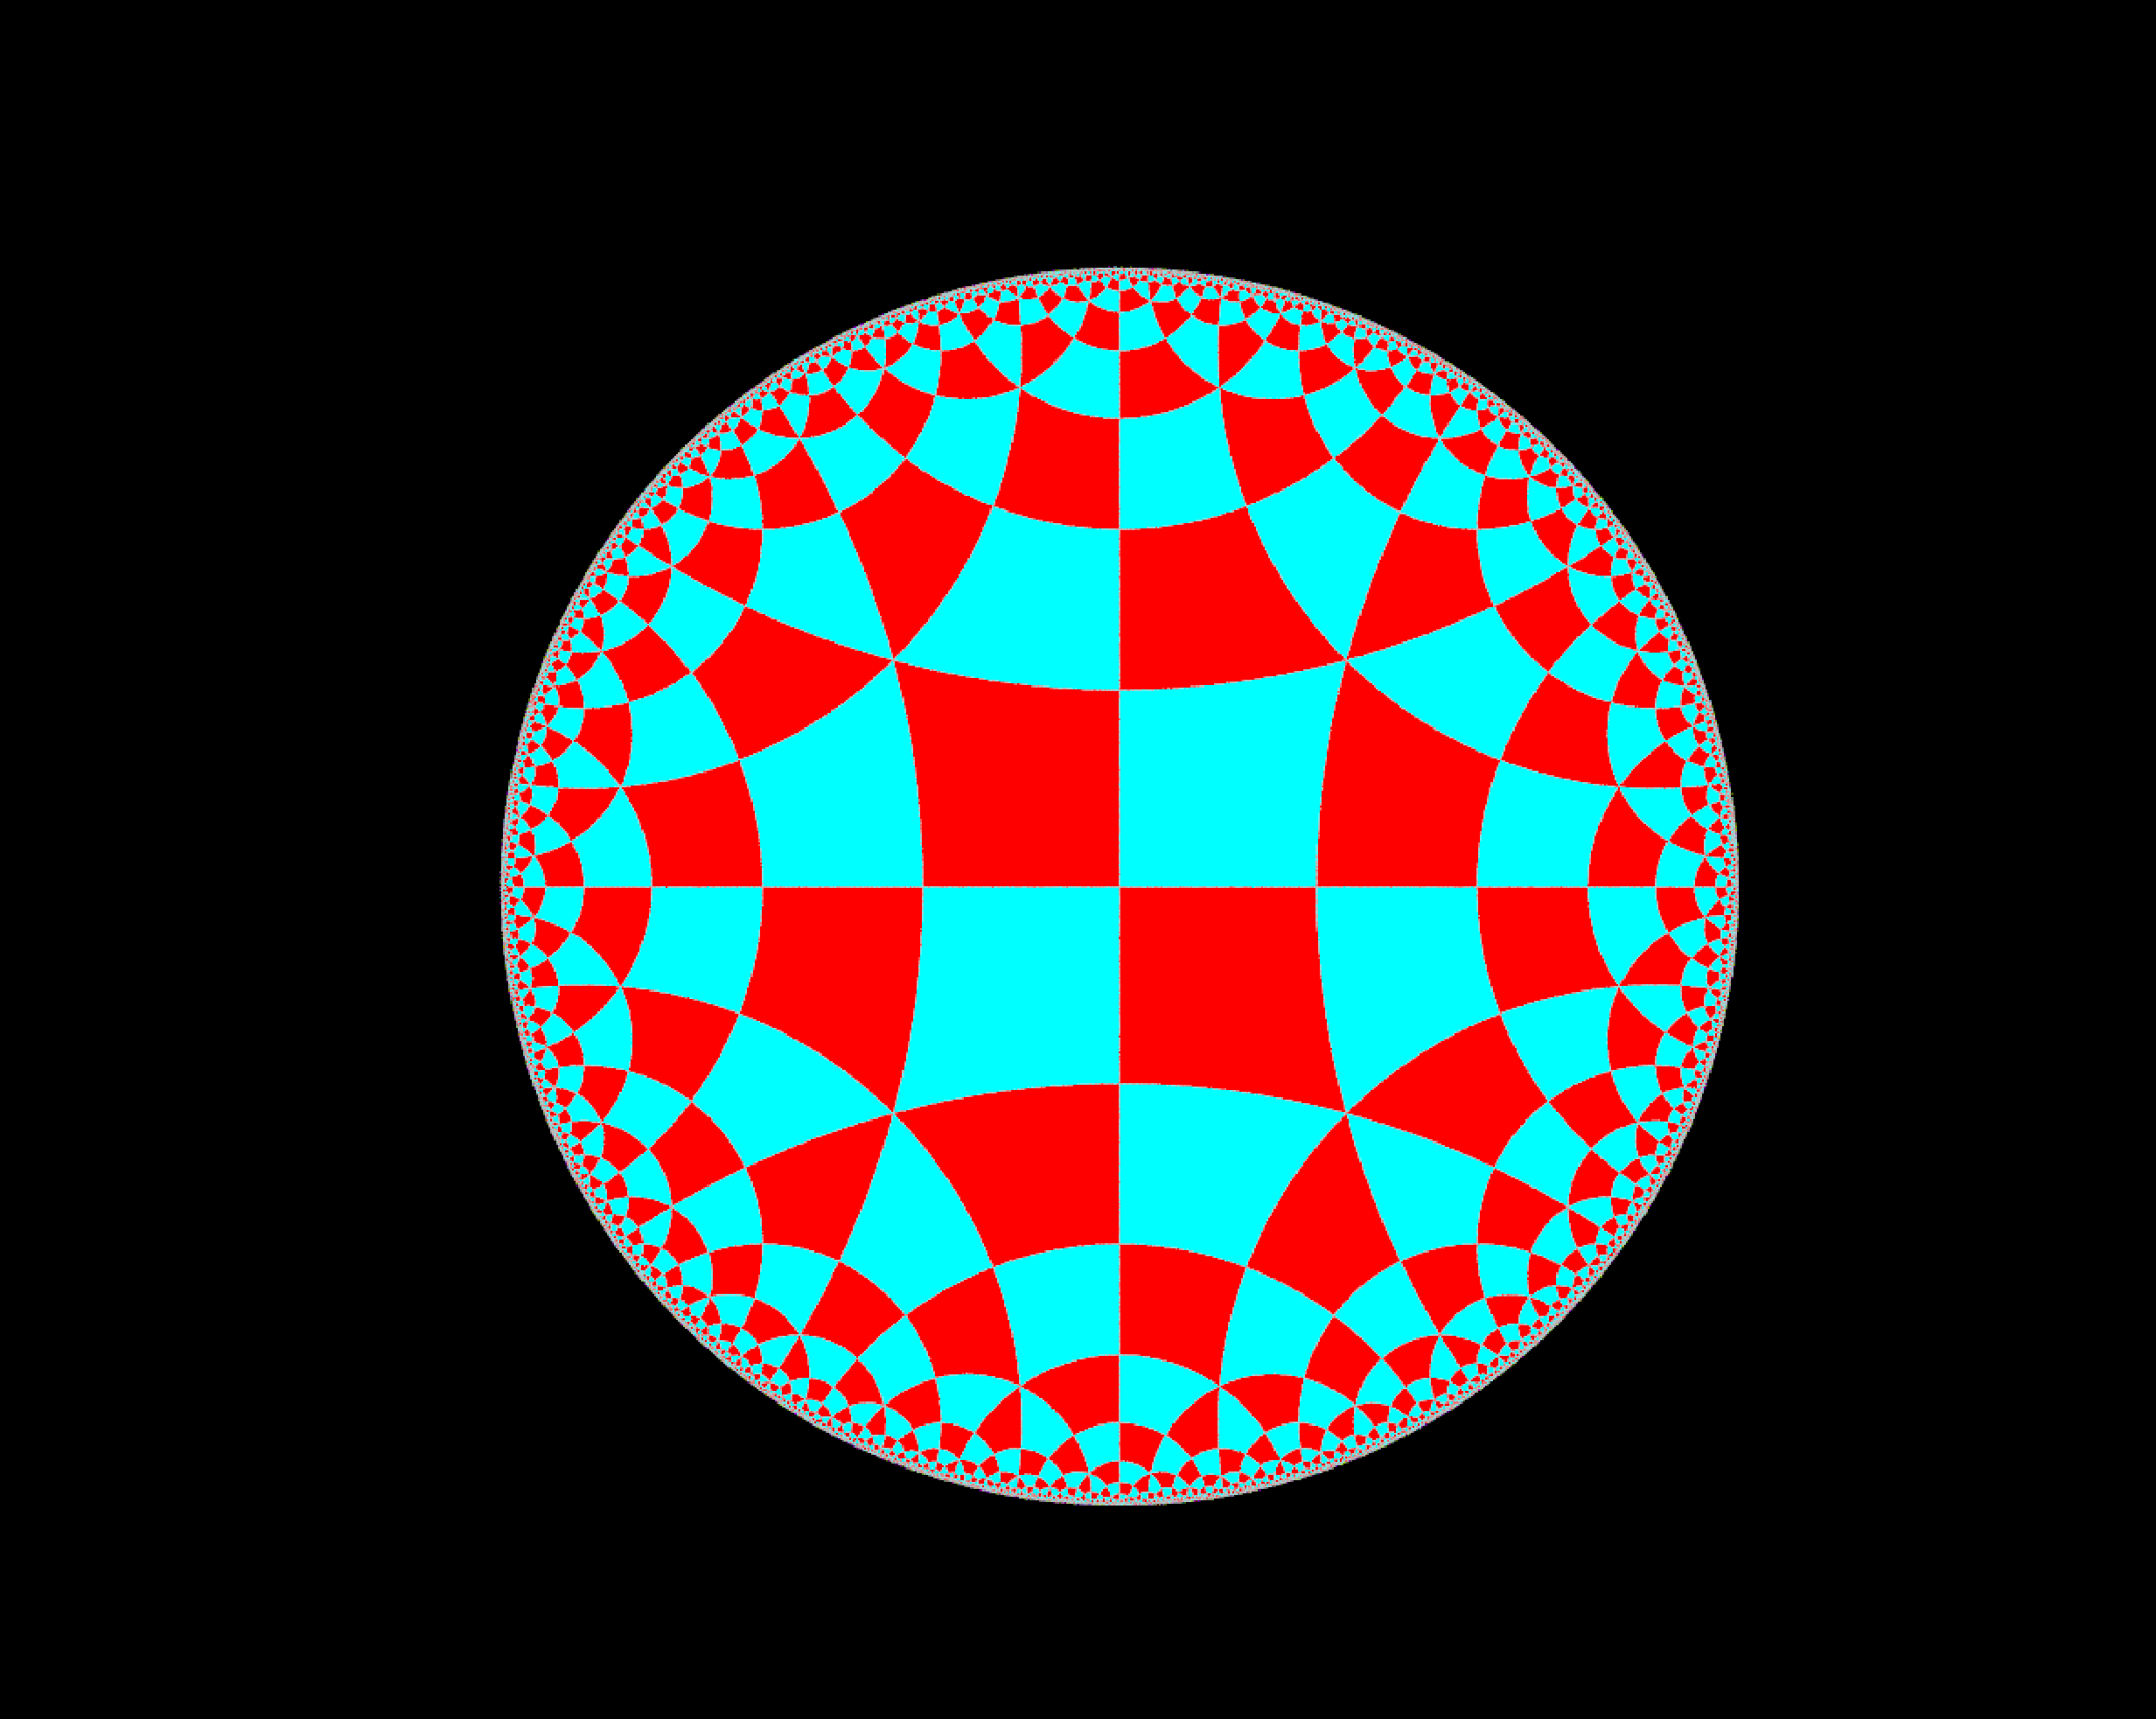
\includegraphics[width=3in, height=3in,
  keepaspectratio]{../img/tessellation/hyperbolicTessellation.pdf}
  \subcaption{Disk model}
  \label{fig:disk}
 \end{minipage}
 \hspace*{\fill}
 \begin{minipage}{0.49\hsize}
  \center
  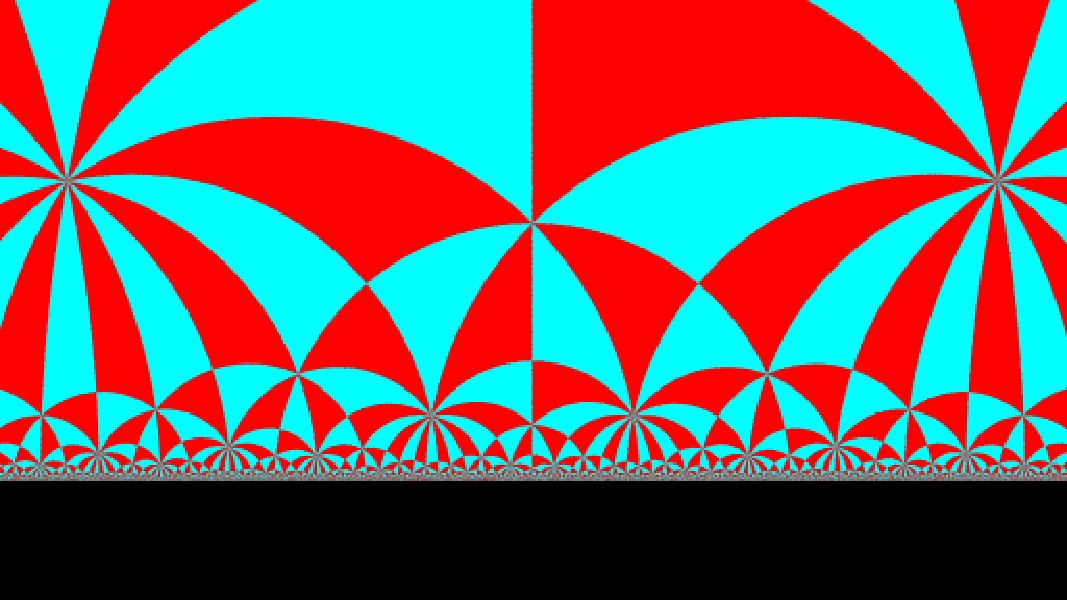
\includegraphics[width=3in, height=3in, keepaspectratio]{../img/tessellation/upperHalf.pdf}
  \subcaption{Half-plane model}
  \label{fig:upperHalf}
 \end{minipage}
  \caption{Hyperbolic Tessellation}
  \label{fig:hyperbolicTessellation}
\end{figure}

これより,図\ref{fig:disk}に示した円盤モデルにおけるテセレーションを描く方法をみていく.
円盤モデルの円盤は単位円とする.
基本タイルを中央にある四つの最も大きなタイルの内の一つとする.
このタイルはX軸,Y軸,そして二つの円弧で囲まれている.
これらの弧に関する反転の組み合せによって基本タイルを動かすと,その軌道は
円周に収束していき,図\ref{fig:hyperbolicTessellation}のような敷き詰め模
様を得ることができる.

双曲テセレーションも前述の方法と同様にして,シェーダで描画することができ
る.図\ref{fig:outer}にシェーダで描画したものを示した.
実は円盤の外側にも世界は広がっており,それは円盤の内側と反転で
移りあう.
円盤の内側に属する点は内側の基本タイルに,円盤の外側に属する点は外側の基
本タイルに移るため,最終的な点の位置で両者を区別することができる.
双曲タイリングは木構造の探索によって計算しようとすると,計算量が多くな
るため,円盤の端まで描画することは難しい.しかし,前述のアルゴリズムを用いると
図\ref{fig:zoom}のように端までリアルタイムで描画することができる.

図\ref{fig:outer}では基本タイルとして,三つの角が$\frac{\pi}{2}$,残りの
角が$\frac{\pi}{3}$である四辺形を用いた.しかし,どのような基本タイルでも敷き
詰めることができるわけではない.
双曲平面において敷き詰めることのできるタイルの条件は\emph{ポアンカレの張
り合わせ定理}として知られている.
例えば,双曲平面における三角形である双曲三角形のテセレーション条件は以下のよう
になる.
\begin{eqnarray*}
3\text{内角を}\frac{\pi}{p},~\frac{\pi}{q},~\frac{\pi}{r}~(p,~q,~r~\in
 \mathbb{N} \cup \{\infty\}) \text{とする時,}~
 \frac{1}{p} + \frac{1}{q} + \frac{1}{r} < 1 \text{を満たす.}
\end{eqnarray*}
このような双曲三角形を二つ張り合わせることで敷き詰め可能な双曲四辺形を得
ることもできる.
図\ref{fig:failed}にはこの条件を満さない双曲三角形の敷き詰めを描いた.
よく見ると一部のタイルが正しく移りあっていないことがわかる.

Vladimir Bulatovは円盤における双曲テセレーションを
図\ref{fig:deformed}のように変形させる方法を考案した
\cite{bridges2013-167}~\cite{bridges2011-479}.
Bulatovは他にも双曲平面や双曲空間におけるテセレーションや,その変形につ
いてまとめている
\footnote{Bulatov Abstract Creations:~
\url{http://bulatov.org/math/index.html}}.
また,Chamberlain Fongは円を正方形に変形させるような擬等角写像を用いて,
双曲テセレーションを矩形に変形する方法をまとめている
\cite{bridges2016-179}.
筆者は双曲テセレーションとその変形を行うウェブアプリケーションを開発している
\footnote{Hyperbolic Tessellator:~
\url{https://soma-arc.net/HyperbolicTessellator/}}.

\begin{figure}[htbp]
  \begin{minipage}{0.49\hsize}
   \center
   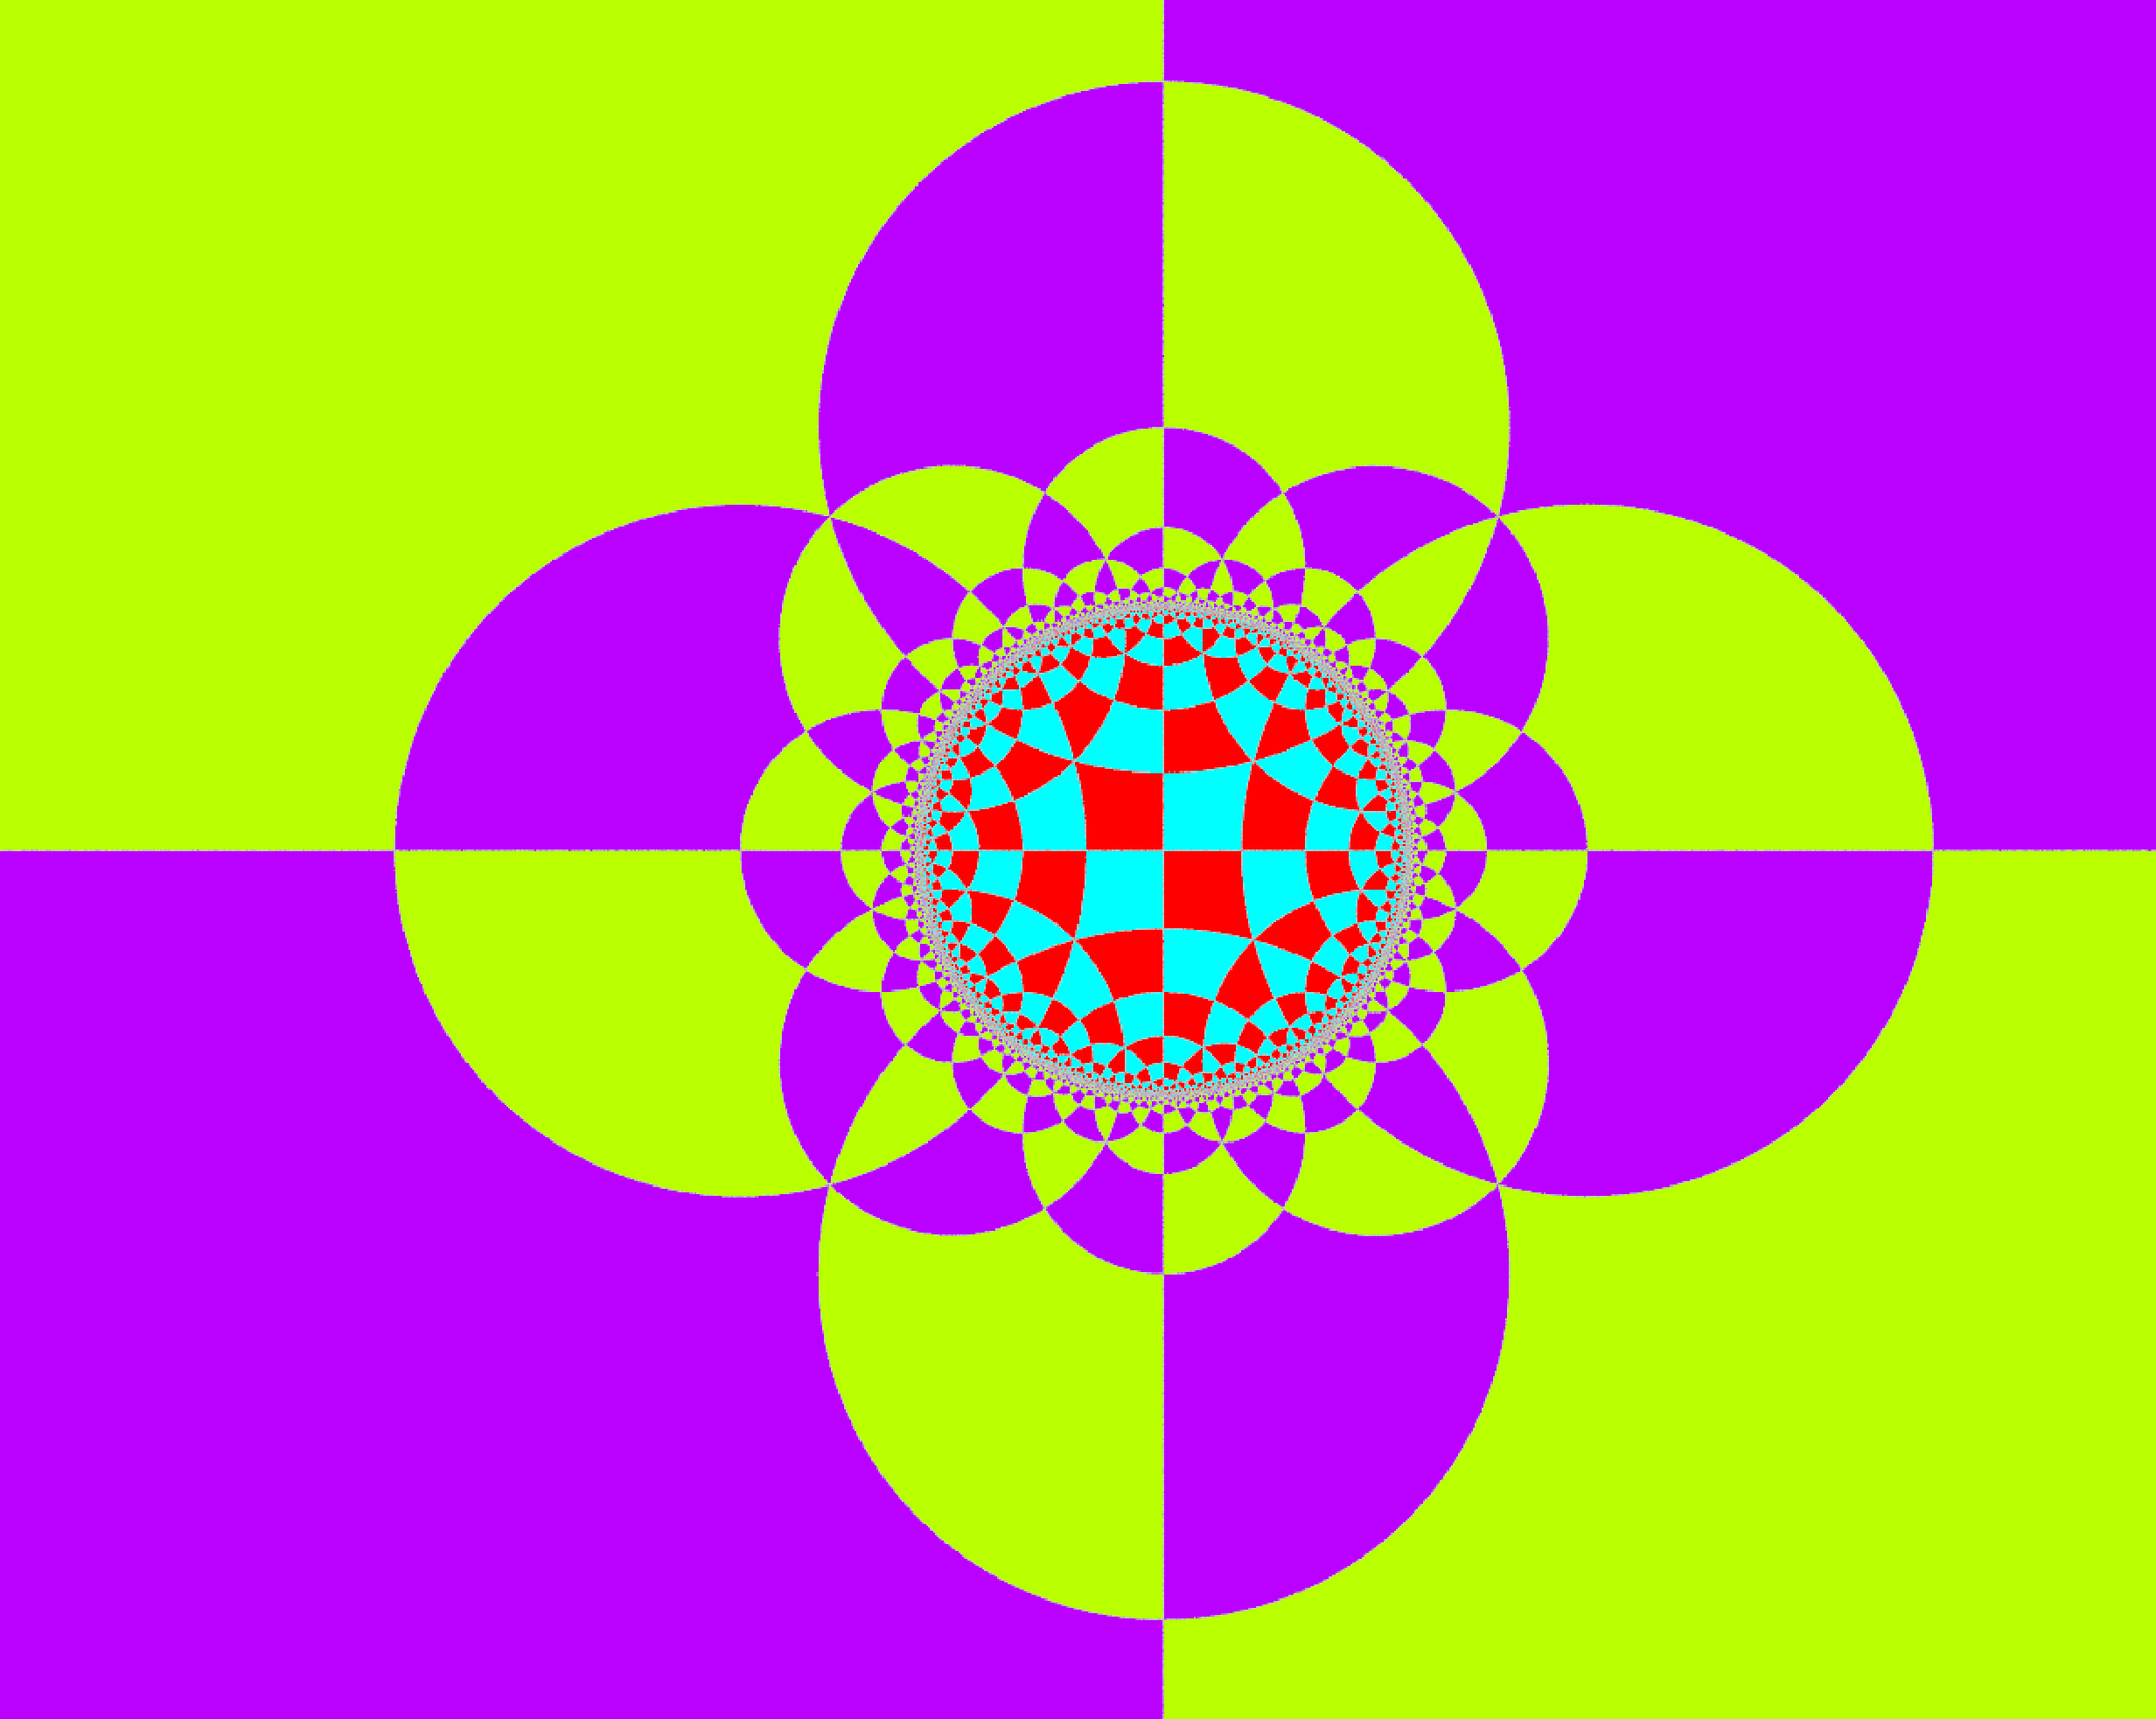
\includegraphics[width=3in, height=3in, keepaspectratio]{../img/tessellation/outer.pdf}
   \caption{Hyperbolic tessellation rendered with shader}
   \label{fig:outer}
  \end{minipage}
 \hspace*{\fill}
 \begin{minipage}{0.49\hsize}
  \center
  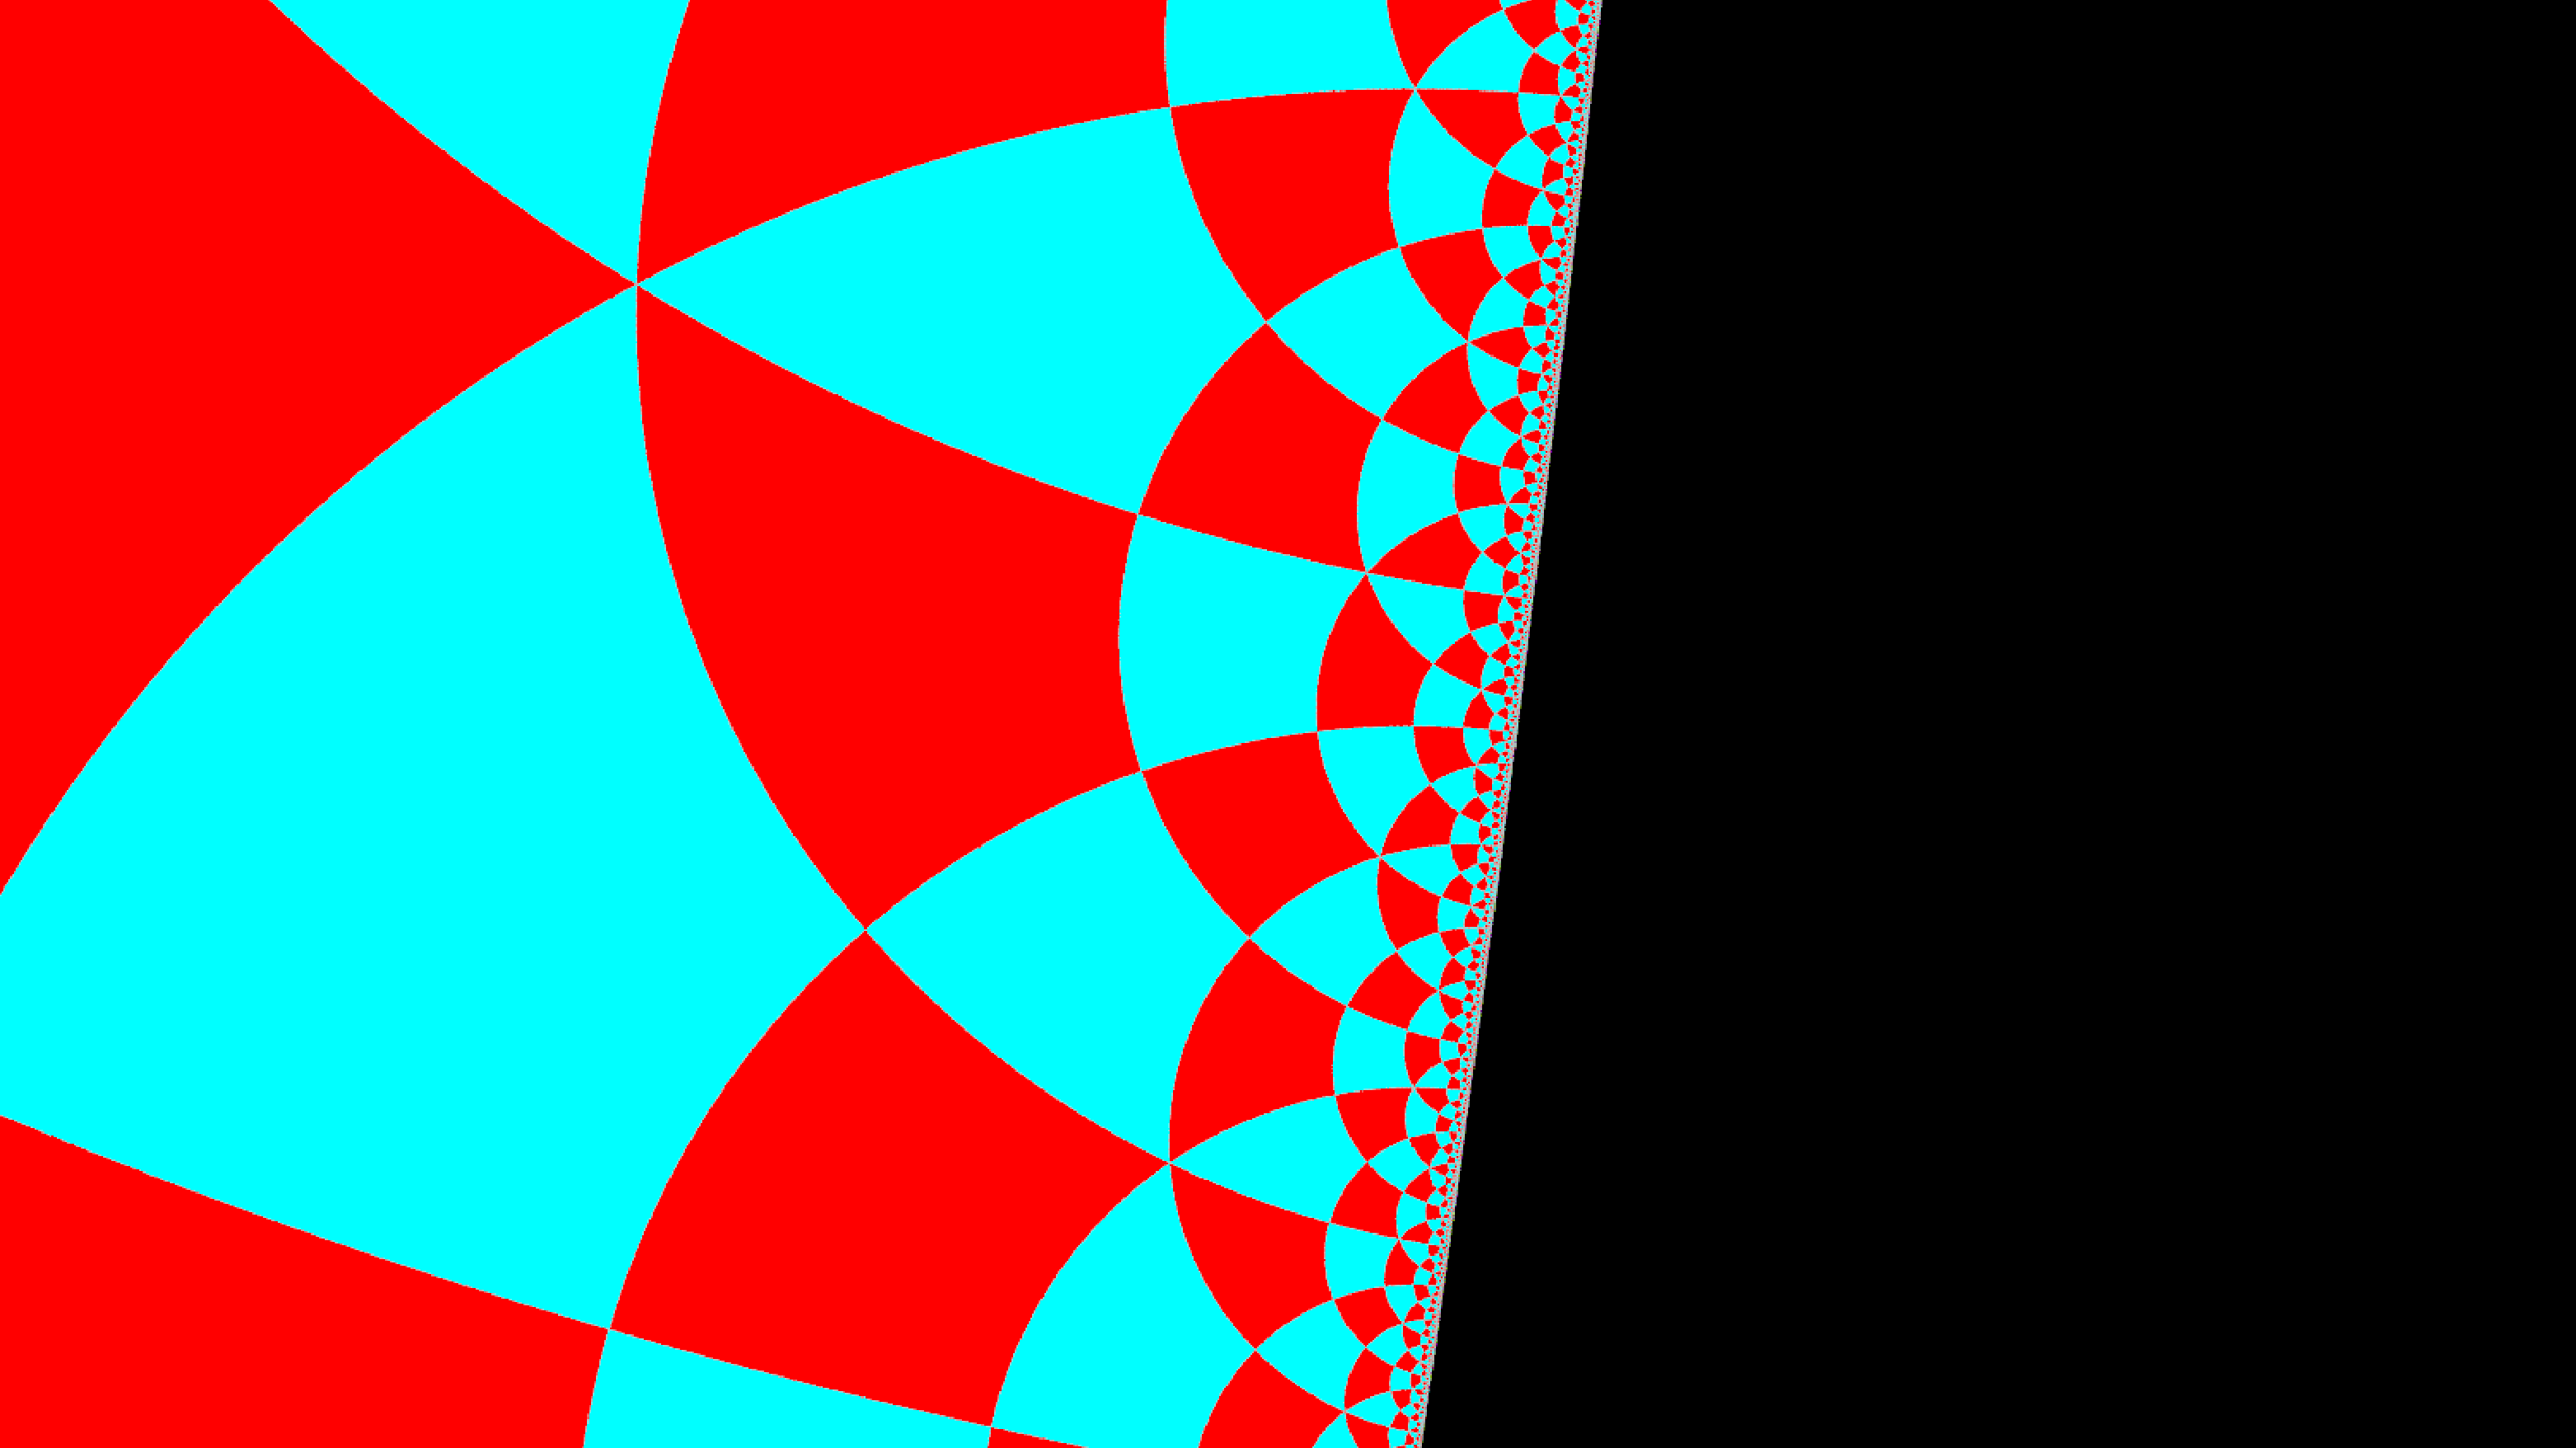
\includegraphics[width=3in, height=3in, keepaspectratio]{../img/tessellation/zoom.pdf}
  \caption{Edge of the disk}
  \label{fig:zoom}
 \end{minipage}
\end{figure}

\begin{figure}[htbp]
  \begin{minipage}[t]{0.49\hsize}
   \center
   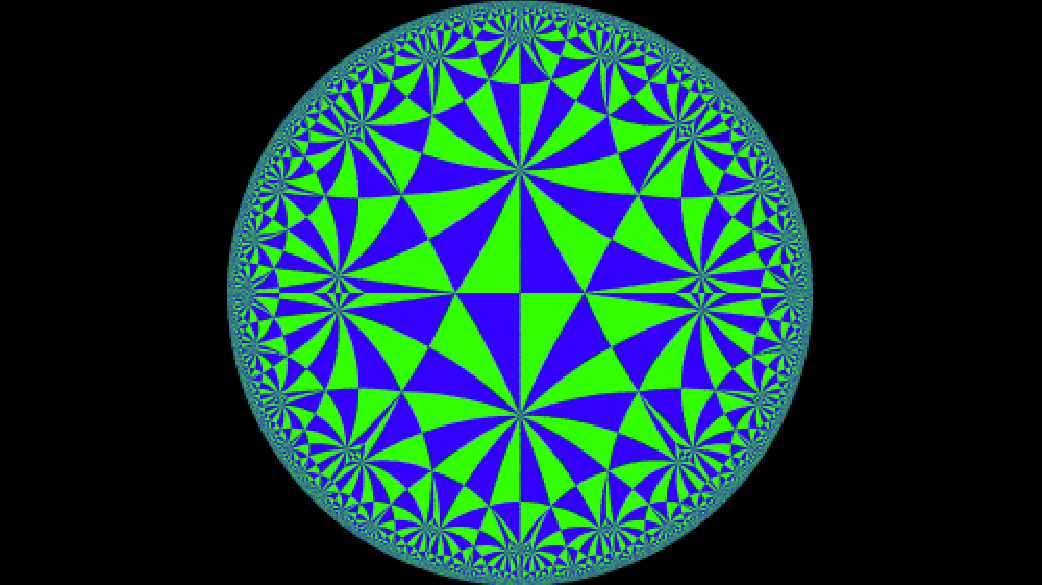
\includegraphics[width=3in, height=3in, keepaspectratio]{../img/tessellation/failed.pdf}
   \caption{Attempt to tessellate non-rational angled hyperbolic triangle}
   \label{fig:failed}
  \end{minipage}
 \hspace*{\fill}
 \begin{minipage}[t]{0.49\hsize}
  \center
  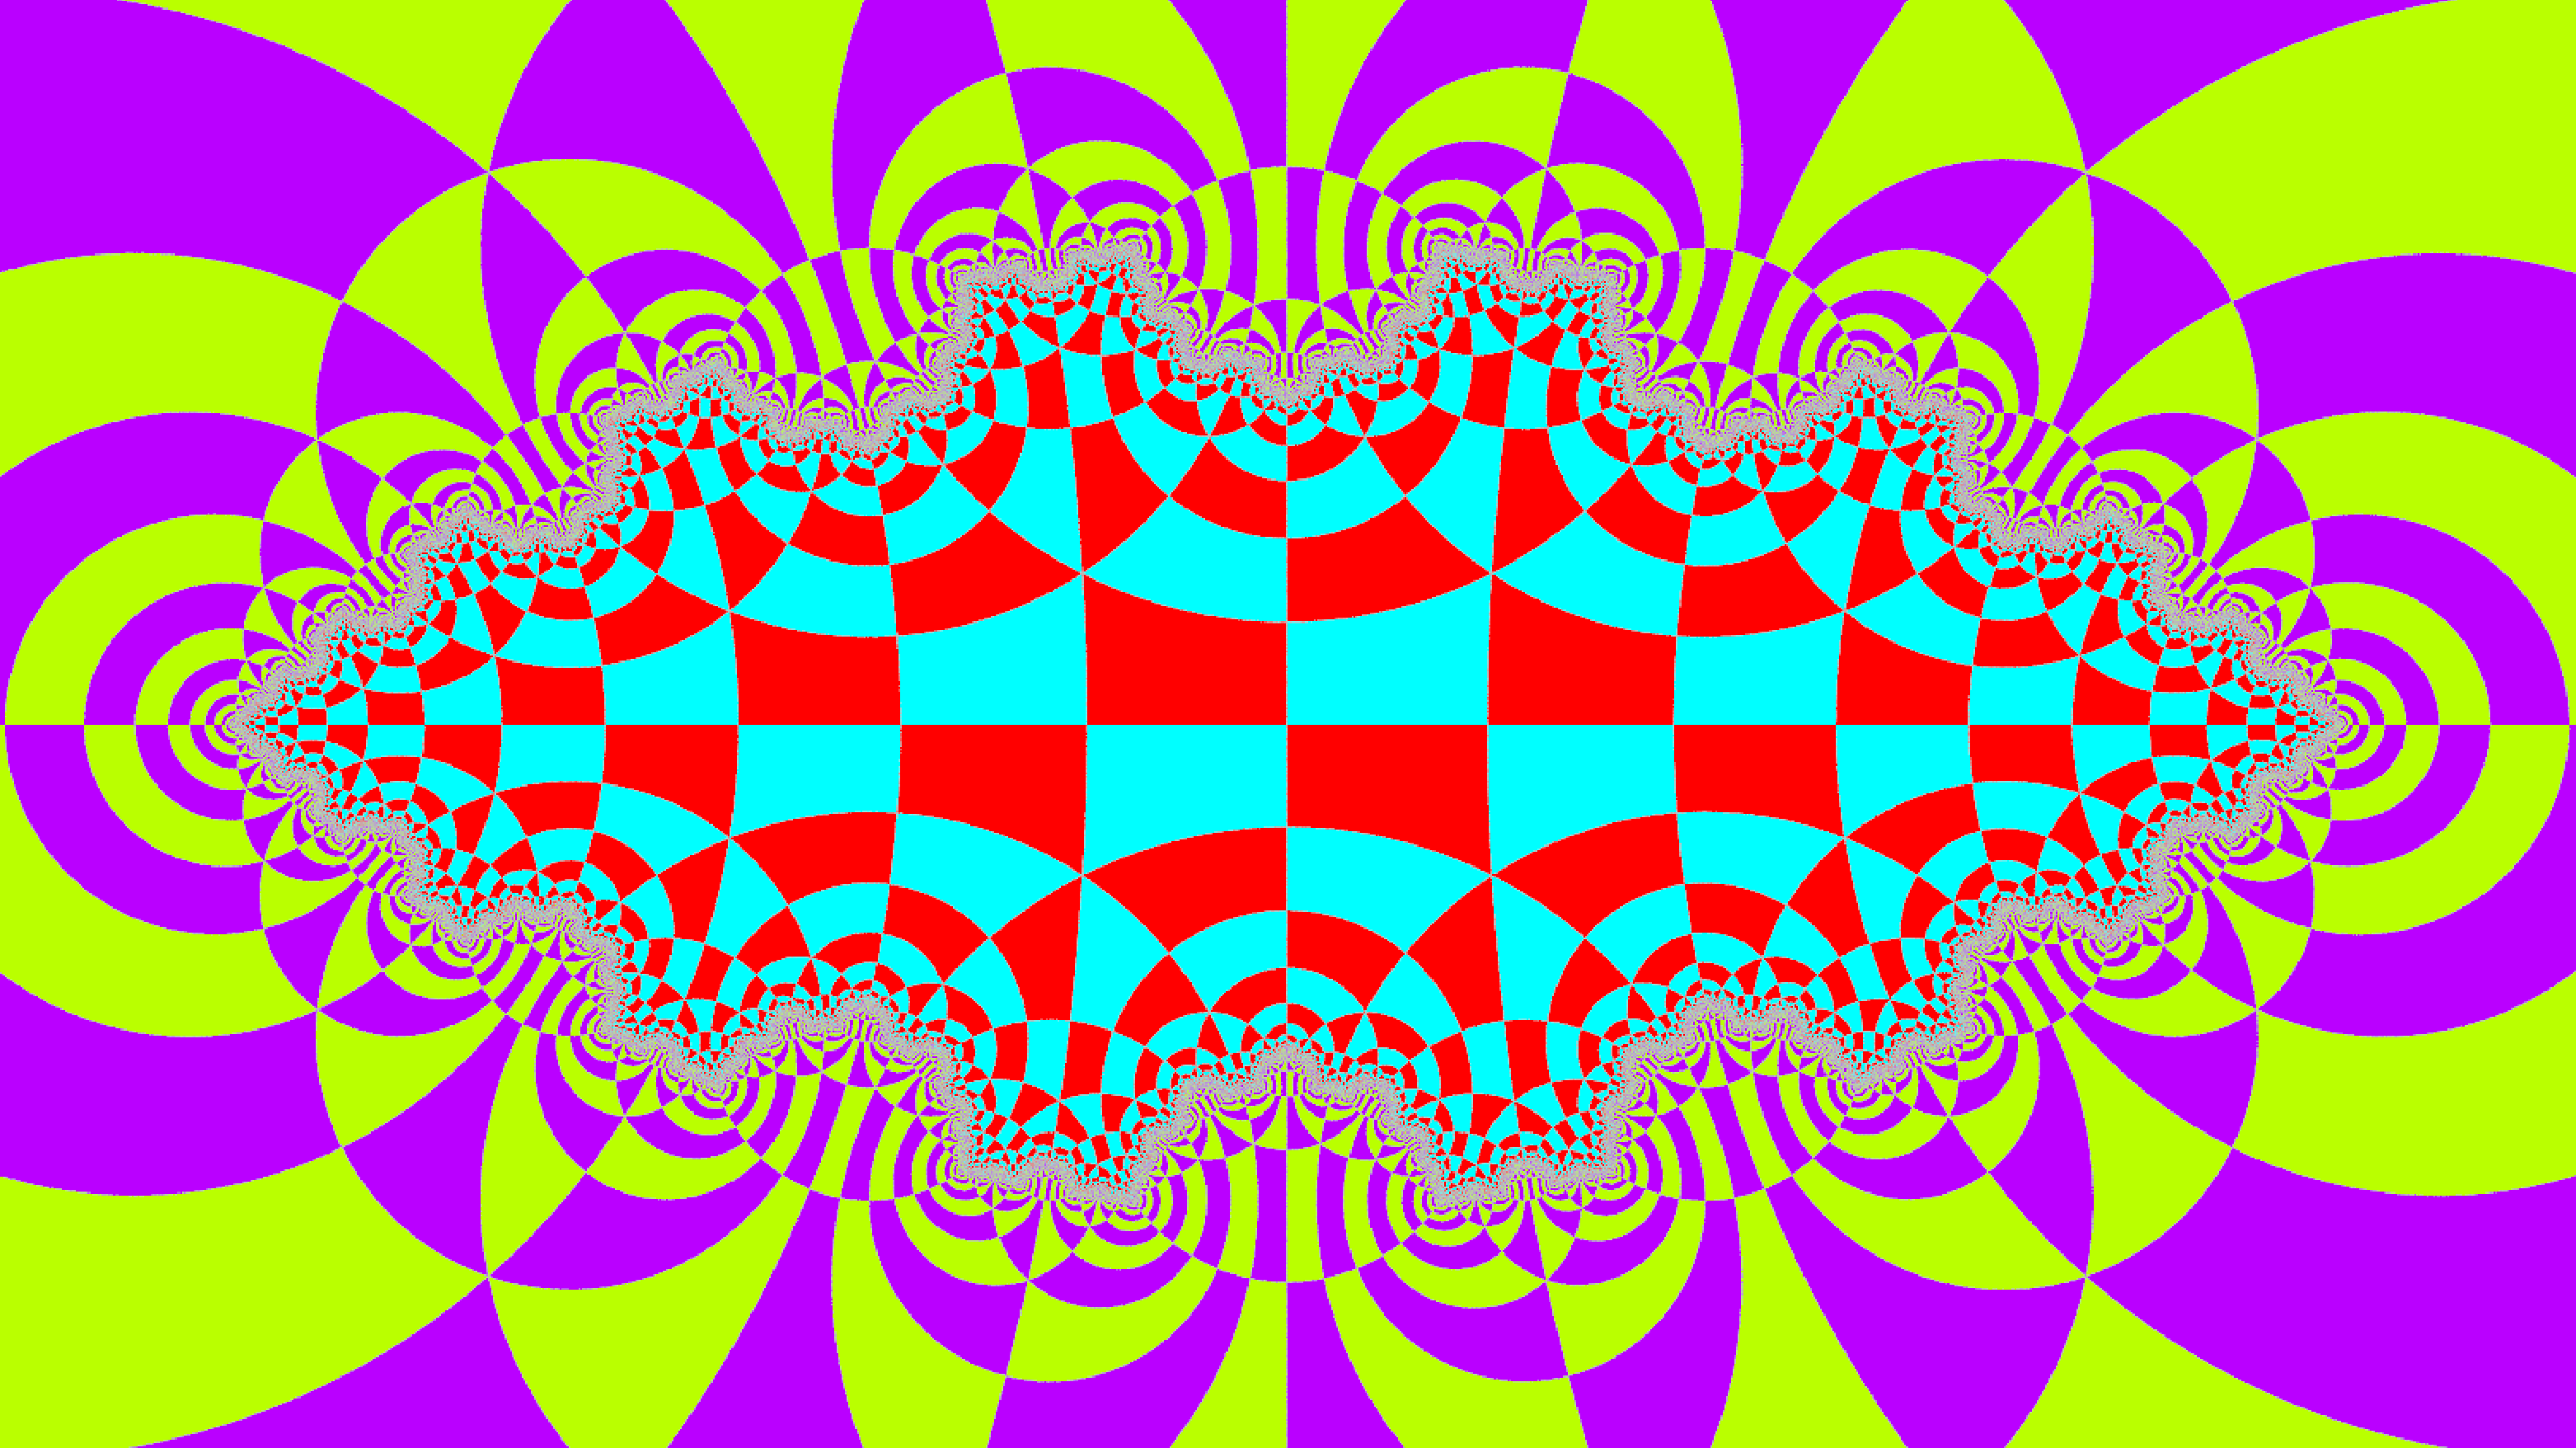
\includegraphics[width=3in, height=3in, keepaspectratio]{../img/tessellation/deformed.pdf}
  \caption{Deformed hyperbolic tessellation}
  \label{fig:deformed}
 \end{minipage}
\end{figure}

\clearpage